% Circle
\begin{figure}[H]
\centering
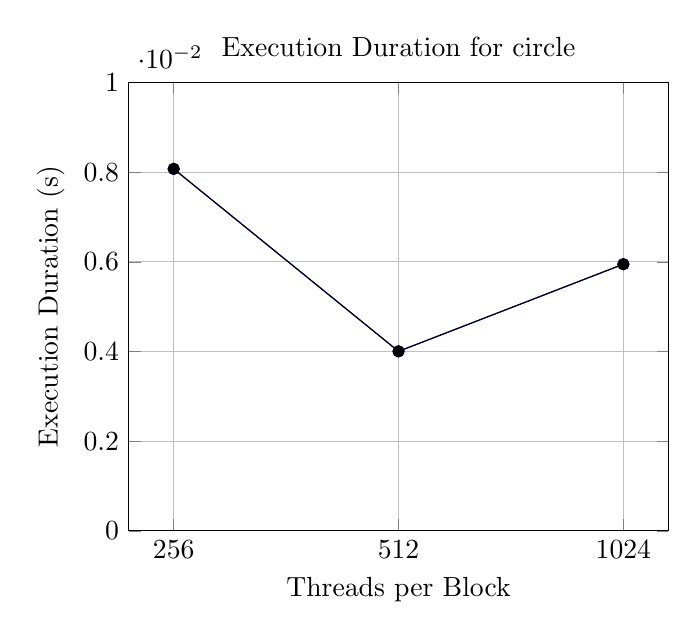
\begin{tikzpicture}
    \begin{axis}[
        xlabel={Threads per Block},
        ylabel={Execution Duration (s)},
        symbolic x coords={256, 512, 1024},
        xtick=data,
        ymin=0, ymax=0.01,
        grid=major,
        title={Execution Duration for circle}
    ]
        \addplot coordinates {(256,0.00807322) (512,0.00400282) (1024,0.00594739)};
        \addplot[mark=*] coordinates {(256,0.00807322) (512,0.00400282) (1024,0.00594739)};
    \end{axis}
\end{tikzpicture}
\caption{Comparison of execution duration for the dataset Circle: N4000 with different
threads per thread block. Experiments are conducted on an NVIDIA RTX4070 consumer GPU}
\end{figure}

